\documentclass[12pt]{article}
\usepackage[utf8]{inputenc}
\usepackage{amsmath,amssymb}
\usepackage{unicode-math}
\usepackage[T2A]{fontenc}
\usepackage[russian]{babel}
\usepackage{graphicx}
\usepackage{subfigure}
\usepackage{subcaption}
\usepackage{url}
\usepackage{float}



\DeclareGraphicsExtensions{.pdf,.png,.jpg}
\usepackage{hyperref}
\usepackage{wrapfig}
\usepackage[left=20mm, top=20mm, right=10mm, bottom=20mm]{geometry}

\usepackage{amsmath} 
\usepackage{amsfonts} 
\usepackage{amssymb} 
\usepackage{wasysym} 
\usepackage{fancyhdr}

\pagestyle{fancy}
\fancyhf{}
\lhead{Семинары 11 и 12. Элементарные частицы.}
\rhead{\textit{Клименок К.Л., МФТИ 2020}}
\rfoot{\thepage}



\begin{document} 
\title{\textbf{Семинары 11 и 12. Элементарные частицы. Сильное и слабое взаимодействие.}}
\author{\textbf{Клименок Кирилл Леонидович}}
\date{25.11.2020}
\maketitle
\textit{Disclaimer} Я не занимаюсь физикой частиц и не являюсь специалистом в этой области.
\section{Теоретическая часть}
Вот и мы дошли до последних двух семинаров, где мы спускаемся еще глубже и начинаем говорить о том, что из себя представляют нуклоны и как они могут существовать в таком виде. И здесь я сделаю небольшую остановку и немного поговорю про механизм работы электромагнитного взаимодействия. Я надеюсь, что вы помните модель из курса электричества, когда 2 заряда чувствовали друг друга через поле которое они создавали. В случае микромира мы используем немного другую модель, а именно модель виртуальных частиц. Идея очень простая: чтобы почувствовать друг друга частицы обмениваются чем-то виртуальным (какими-то частицами переносчиками взаимодействия). Вопрос как такое возможно отпадает сам собой, если мы вспомним соотношение неопределнностей энергии-времени в трактовке нарушения закона сохранения. Отсюда можно оценить характерное время жизни таких переносчиков с массой $m$:
\begin{equation*}
    \tau \approx \dfrac{\hbar}{mc^2}
\end{equation*}
Тогда эта модель работает и для фотонов, ведь они безмассовые и могут существовать сколь угодно долго и переносить электромагнитное взаимодействие на любые расстояния.
\subsection{Стандартная модель}
Итак мы договорились о языке виртуальных частиц, а теперь можно выкатить вам на суд сумму всех знаний о там из чего состоит это зоопарк частиц, которые наблюдали с середины 20 века.
\begin{figure}[h]
    \centering
    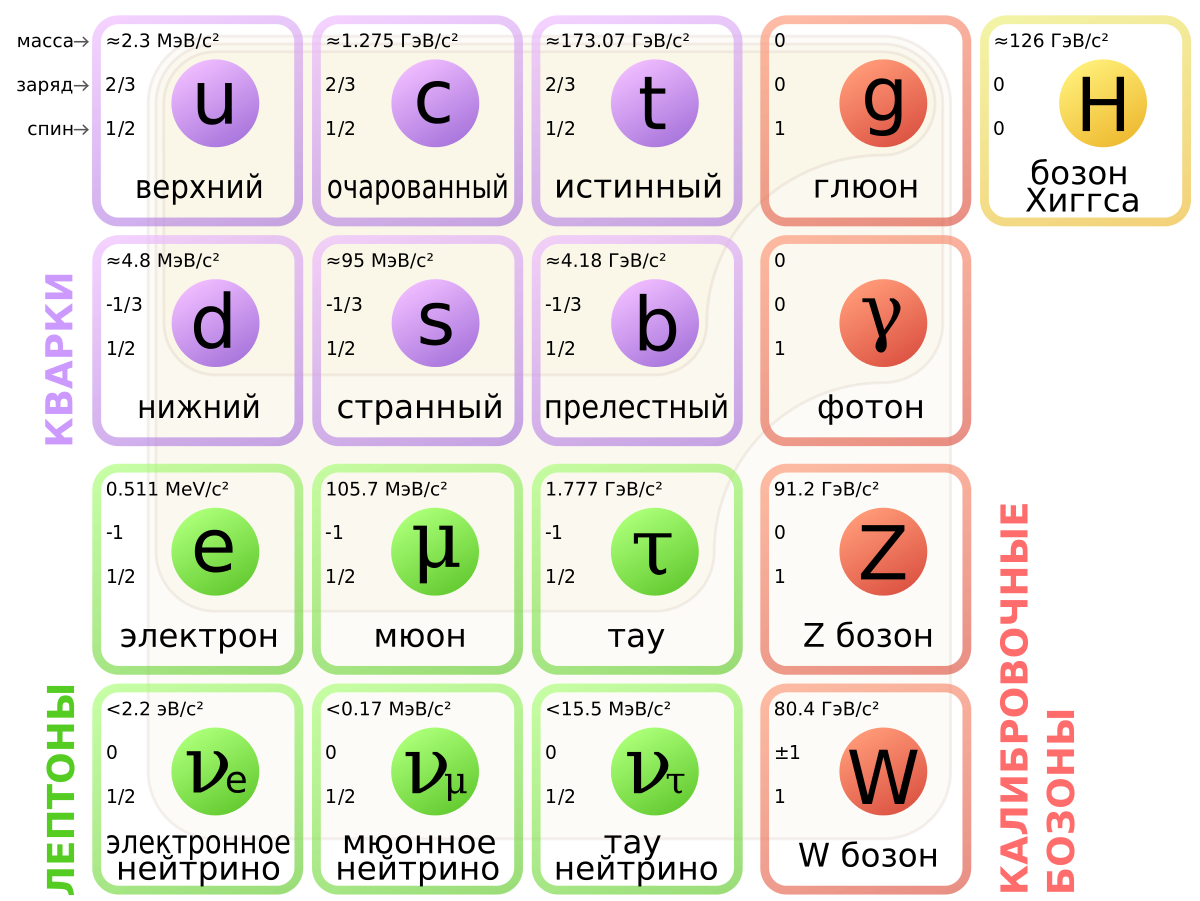
\includegraphics[width=\textwidth,height=\textheight,keepaspectratio]{Seminar_11/pics/pic_01_standart_model.png}
    \caption{Стандартная модель}
    \label{fig:sem_11_model}
\end{figure}

Давайте посмотрим на эту таблицу  на рисунке \ref{fig:sem_11_model}. У нас есть кварки, лептоны, переносчики взаимодействия (<<калибровочные бозоны>>) и немного особняком стоит бозон Хиггса. Еще к кваркам и лептонам есть античастицы. На данным момент это наиболее полная картина мира элементарных частиц. Теперь давайте обсуждать это все более подробно.
\paragraph{Кварки} 
С ними мы сталкиваемся, когда говорим о протонах и нейтронах, а именно об их составных частях. Но сейчас надо немного обобщить наши знания, так как есть целая куча разных частиц из кварков состоящих. Начнем с того, что одиночные  кварки сами по себе не были обнаружены, а только в составе \textbf{\textit{адронов}} --- частиц из 2 или 3 кварков (мы не рассматриваем экзотику типа пентакварка). Частицы из 2 кварков называются \textit{\textbf{мезоны}} и именно они, в частности, переносят взаимодействие в ядре, а частицы из 3 кварков --- \textit{\textbf{барионы}}, именно к ним и относятся протоны и нейтроны. Что еще видно из стандартной модели, так это заряды, выраженные в долях заряда электрона и спины, которые равны $1/2$. И если заряды в принципе не дают нам что-то новое, то вот наличие полуцелого спина дает нам принципиально новый результат из-за принципа Паули. Получается, что есть новая характеристика, которая ранее не наблюдалась но присуща именно кваркам и различает их. Эту характеристику называют <<цветовым зарядом>>, или просто цветом, и он может быть <<красным>>, <<зеленым>>, <<синим>> и их антицветами. При этом любой адрон всегда белый (состоит из 3 разных цветов, 3 разных антицветов или из пары цвет-антицвет).Также, для различных реакций работает <<закон сохранения барионного заряда>>, то есть в рамках одного процесса количество барионов сохраняется до и после реакции.
\paragraph{Лептоны}
К ним нужно относиться как к истинно элементарным частицам и мы их в принципе уже знаем из $\beta$-распада. Самое главное, что про них надо знать, что они никогда не появляются по одиночке, или, другими словами, должен работать закон сохранения <<лептонного заряда>>. Он работает по поколениям и имеет знак $-1$ для частиц соответствующего поколения, знак $+1$ для античастиц этого же поколения и $0$ для остальных поколений лептонов. Именно поэтому при вылете электрона в $\beta$-распаде получается еще и анти электронное нейтрино.
\paragraph{Калибровочные бозоны}
Это просто переносчики взаимодействия. Глюон переносит сильное взаимодействие, фотон -- электромагнитное. Они оба безмассовые. А вот W и Z бозоны нужны для слабого взаимодействия и их масса уже на равна нулю.

\subsection{Сильное взаимодействие}
Давайте посмотрим как, в рамках текущего представления, работает сильное взаимодействие между кварками. Картинка \ref{fig:sem_11_quark} достаточно понятна сама по себе. У нас есть барион, который стабильно живет с кварками разных цветов, затем один из них, как в примере синий, <<выпускает>> глюон таким образом, что он состоит из 2 цветов синего и антизеленого, а сам меняет цвет на зеленый. Этот глюон летит к другом зеленому кварку и поглощается, что изначальный зеленый и анти зеленый из глюона взаимно уничтожаются, а сам кварк становится синим.
\begin{figure}[h]
    \centering
    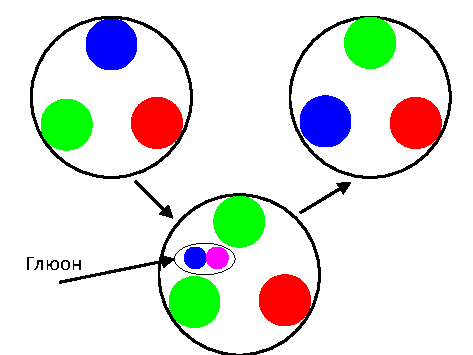
\includegraphics[width=0.6\textwidth,height=\textheight,keepaspectratio]{Seminar_11/pics/pic_02_stong.pdf}
    \caption{Механизм обмена глюонами внутри бариона}
    \label{fig:sem_11_quark}
\end{figure}

И вот тут пришло время поговорить о понятии <<конфайнмент>> и <<асимптотическая свобода>>. Как я уже говорил, свободных одиночных кварков и глюонов мы не наблюдаем, поэтому предположили следующее объяснение. Пусть цветовой заряд, которым обладают кварки, имеет свойство так называемого <<антиэкранирования>>. Антиэкранирование происходит из-за того, что глюоны сами обладают цветовым зарядом и в процессе движения как бы <<порождают новые глюоны из вакуума>> и тем усиливают взаимодействие. В результате кварки притягиваются тем сильнее, чем дальше они друг от друга. Это и есть конфайнмент. а свободными кварки могут стать только, когда расстояние между ними стремится к нулю, а это и есть асимптотическая свобода. Отсюда, кстати, очень легко понять как можно рассматривать столкновения на больших энергиях различных частиц, зная их кварковый состав. получается, что мы должны просто рассмотреть сечение каждого кварка на каждом кварке и все, так как энергия их связи будет много меньше энергии связи столкновения и это все равно что рассмотреть столкновение одной группы  свободных шариков на другой группе таких же шариков.

Теперь <<понимая>> это можно сказать как нуклоны сосуществуют в ядре. Для этого у нас есть картинка \ref{fig:sem_11_nuclei}. На ней есть нейтрон, у которого один из D-кварков отходит от остальных и образуется глюооная трубка, в которой сосредотачивается большая энергия (асимптотическая свобода наоборот) и в результате из вакуума у нас появляется пара U  и анти U кварки (то самое нарушение закона сохранения энергии на малых масштабах времени). В результате U кварк объединяется с исходными 2 и нейтрон становится протоном, а анти U кварк объединяется с В кварком и они становятся мезоном, который летит к другому адрону, где анти кварк из мезона аннигилирует с кварком из нуклона и D кварк занимает его место.

\begin{figure}[h]
    \centering
    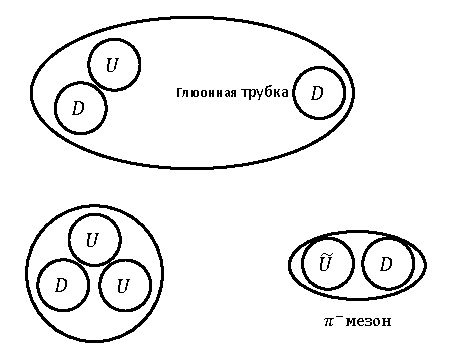
\includegraphics[width=0.6\textwidth,height=\textheight,keepaspectratio]{Seminar_11/pics/pic_03_nuclei.pdf}
    \caption{Механизм внутриядерного взаимодействия}
    \label{fig:sem_11_nuclei}
\end{figure}

\subsection{Слабое взаимодействие}
В эту категорию исторически попадало все странное, что никак не описывалось сильным или электромагнитным взаимодействиями. Из того, с чем мы столкнемся в задачах с вами это преобразование кварков в рамках реакций или вылет лептонов, в частности тот самый $\beta$-распад как раз происходит по механизму слабого взаимодействия. Схема превращения кварков представлена на рисунке \ref{fig:sem_11_weak}. Еще одна особенность, про которую я заикался ранее, в слабом взаимодействии не сохраняется четность. 
\begin{figure}[h]
    \centering
    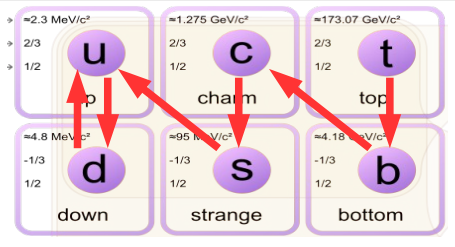
\includegraphics[width=0.4\textwidth,height=\textheight,keepaspectratio]{Seminar_11/pics/pic_04_weak.PNG}
    \caption{Механизмы превращения кварков}
    \label{fig:sem_11_weak}
\end{figure}

\subsection*{Диаграммы Фейнмана*}
Это красивый и удобный инструмент для того, чтобы показывать что и как происходит в различных процессах с элементарными частицами, придуманный Ричардом Фейнманом. Общие идея такова, что схема читается слева на право, как направлено время. Стрелки соответствуют тому, частица это (стрелка в направлении хода времени) или античастица( против хода времени). Типы стрелок соответствуют тому, реальная ли это частица или переносчик взаимодействия. А в каждой точке пересечения диаграммы выполняются законы сохранения. Вот пример на рисунке \ref{fig:sem_11_fey}. Слева --- электрон взаимодействует с позитроном, просто притягиваются. А справа аннигиляция с последующим образованием пары.
\begin{figure}[h]
    \centering
    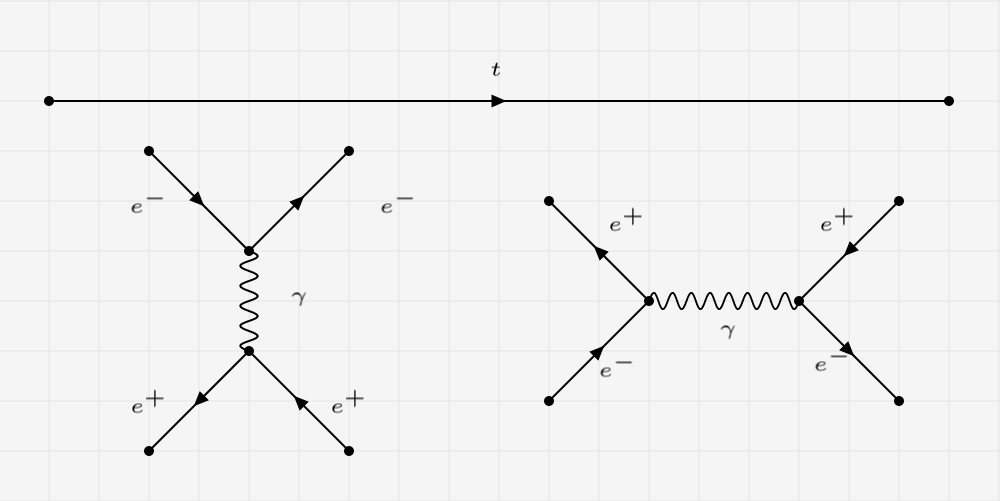
\includegraphics[width=0.8\textwidth,height=\textheight,keepaspectratio]{Seminar_11/pics/pic_05_fey.PNG}
    \caption{Примеры фейнмановских диаграмм}
    \label{fig:sem_11_fey}
\end{figure}

\section{Практическая часть}
\subsection{Задача 10.7}
\label{task_}
\paragraph{Условие}
Указать какие из реакций возможны.
\paragraph{Решение}
Общие замечания по тому на что смотреть и как решать. Во-первых, непонятные греческие буквы это разные адроны. Их кварковый состав можно посмотреть в конце задачника в приложении 6. Во-вторых, надо определиться что это за взаимодействие сильное, слабое  или электромагнитное. Для сильного взаимодействия у нас сохраняется количество барионов и могут появляться только пары кварк-антикварк, для слабого кварки более высоких поколений меняются на кварки более низких поколений (рисунок \ref{fig:sem_11_weak}), а электромагнитное вообще идет без смены состава. Теперь реакции:
\begin{enumerate}
    \item $\Sigma^+ \rightarrow \pi^+ + n$. Переписываем в терминах кварков: $uus \rightarrow u\widetilde{d} + udd$. Тут у нас распался странный кварк из второго поколения в первое, это нормально, а потом появились $d$ и $\widetilde{d}$ кварки, что в принципе нормально. Такая реакция возможна в рамках слабого взаимодействия.
    \item $\Sigma^- + p\rightarrow \pi^0 + \widetilde{K^0}$. Переписываем в терминах кварков: $dds + uud \rightarrow u\widetilde{u} + d\widetilde{d} + \widetilde{d}s$. Тут 2 бариона распались на 3 мезона. По идее это должно быть сильное взаимодействие, но барионный заряд не сохраняется. Такая реакция невозможна.
    \item $\pi^- + p \rightarrow \Lambda + \widetilde{K^0}$. Переписываем в терминах кварков: $ \widetilde{u}d + uud \rightarrow uds + \widetilde{d}s$. По идее это взаимодействие бариона и мезона, но у нас появляются из неоткуда 2 странных кварка, а повышение поколения кварков не работает, поэтому нельзя
    \item $\pi^- + p \rightarrow \Sigma^- + K^+$. Переписываем в терминах кварков: $ \widetilde{u}d + uud \rightarrow dds + u\widetilde{s}$. А вот тут все хорошо --- появились странный и антистранный кварк, количество барионов сохраняется и значит это сильное взаимодействие
\end{enumerate}
Остальные дорешаете сами.

\subsection{Задача 10.60}
\label{task_}
\paragraph{Условие}
Резонансы $\Upsilon$ и $\Upsilon^'$ с энергиями покоя $E_1 = 9.46$ ГэВ и $E_2 = 10.02$ ГэВ можно считать основным и первым возбужденным состояниями боттомония, мезона с кварковым составом $b\widetilde{b}$. Пользуясь нерелятивистским приближением и считая потенциал взаимодействия между ними кулоновским $U=-q^2/r$, где $q$ -- цветовой заряд кварка. Оценить массу b-кварка и константу сильного взаимодействия $g^2=q^2/\hbar c$
\paragraph{Решение}
Тут в условии нам явно намекают, что нужно использовать модель водородоподобного атома, так как у нас есть положительный и отрицательный кварки, которые <<вращаются вокруг общего центра масс>>. Единственным отличием будет то, что уровни энергии тогда нужно отсчитывать не от нуля, а от массы невозбужденной частицы. Тогда воспользуемся готовой формулой из 6 семинара для уровней энергии:
\begin{gather*}
    E_n = 2m_bc^2 - \mu\dfrac{q^4}{2\hbar^2n^2}
\end{gather*}
Из условия можем посчитать разность энергий $\Delta E$ для $n=1$ и $n=2$ и составить систему:
\begin{gather*}
    \Delta У = E_2 - E_1 = \dfrac{3}{4}\mu\dfrac{q^4}{2\hbar^2} \Rightarrow \mu\dfrac{q^4}{2\hbar^2n^2} = \dfrac{4}{3}\Delta E\\
    E_1 = 2m_bc^2 - \dfrac{4}{3}\Delta E\\
    E_2 = 2m_bc^2 - \dfrac{1}{3}\Delta E\\
    m_bc^2 = \dfrac{4E_2-E_1}{6} = 5.1 \text{ ГэВ}, g^2=\sqrt{32\Delta E(4E_2-E_1)} \approx 0.8
\end{gather*}

\subsection{Задача 10.70}
\label{task_}
\paragraph{Условие}
При больших энергиях сечение протон-протонного рассеяния равно $\sigma(pp) = 39$ мбн. Принимая во внимание кварковую структуру протона и пиона оценить сечение $\sigma(\pi p)$. Считая, что $\sigma(Kn) = 19$ мбн, найти $\sigma(\Lambda n)$ и $\sigma(\Theta n)$.
\paragraph{Решение}
Вот тут нам как раз и пригодится идея о том, что кварки очень слабо связаны друг с другом по сравнению с энергией при столкновении. Давайте посмотрим кварковый состав для протона и попробуем переписать сечение реакции через сечение взаимодействия отдельных кварков. 

Взаимодействие протон это $uud + uud$, то есть мы получаем всего 9 пар кварк-кваркового взаимодействия: $\sigma(pp) = 4\sigma(uu)+ 4\sigma(ud) +\sigma(dd) = 9\sigma_0$. Такое равенство возможно, так как у нас все кварки 1 поколения и с точки зрения сечения они одинаковы. Тогда для $$\sigma(\pi p) = \sigma(u\widetilde{d} uud)=2\sigma(uu)+ \sigma(ud) + 2\sigma(\widetilde{d}u)+ \sigma(\widetilde{d}d) = 6\sigma_0 = 2\sigma(pp)/3 = 26$$ мбн.

Остальные пары делаются аналогично, но там в составе есть странный кварк 2 поколение и его сечение с кварками 1 поколения отличается, это надо учесть. Я думаю, что такая задача вам по силам.


\subsection{Задача 10.73}
\label{task_}
\paragraph{Условие}
Исходя из законов сохранения дописать реакции между протоном/нейтроном и мюонным нейтрино/антинейтрино. Найти отношение эффективных сечений этих реакций, нарисовать кварковые схемы реакций.
\paragraph{Решение}
Вот тут мы переходим уже к слабому взаимодействию, так как нейтрино это лептоны, а в сильном взаимодействии они не появляются. Тогда этот процесс будет уже внутри нуклонным и нейтрино или антинейтрино будет взаимодействовать с каким-то конкретным кварком. А что тогда будет на выходе и как понять с каким? Очень просто --- для этого используем закон сохранения лептонного заряда, а именно тот его факт,что если слава в реакции есть мюонное нейтрино, тогда справа в реакции должен получиться мюон (для античастиц тоже самое). Дальше Смотрим на закон сохранения заряда: мюон штука отрицательная, значит выбираем в качестве переносчика взаимодействия $W^+$ бозон, что сохранить заряд. А дальше смотрим на рисунок \ref{fig:sem_11_weak} и видим, что в слабом взаимодействии кварки $u$ и $d$ могут переходить только друг в друга. Но заряд бозона у нас положительный и для того чтобы сохранить заряд во взаимодействии с протоном мы должны выбрать именно взаимодействие с его $d$ кварком и перевести его в $u$ кварк. Написано сложно, но давайте нарисуем диаграмму Фейнмана \ref{fig:sem_11_10_73} и все встанет на свои места. Аналогичные рассуждения и для оставшихся трех реакций. И идея с отношением сечений это просто отношение числа тех кварков, с которыми наше нейтрино и будет реагировать.
\begin{figure}[h]
    \centering
    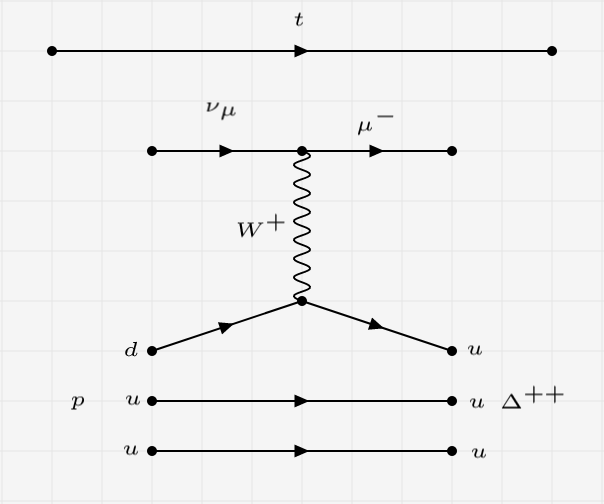
\includegraphics[width=0.8\textwidth,height=\textheight,keepaspectratio]{Seminar_11/pics/pic_06_task_10_73.PNG}
    \caption{Диаграмма Фейнмана для взаимодействия протона и мюонного нейтрино}
    \label{fig:sem_11_10_73}
\end{figure}


\subsection{Задача Т7}
\label{task_}
\paragraph{Условие}
Мюонное нейтрино, попав в жидководородную камеру, рождает промежуточный бозон $W^+$ ($m_Wc^2 = 81$ ГэВ). Найти минимальную энергию нейтрино.
\paragraph{Решение}
Эта задачка по своей сути на релятивистские столкновения, которые вы решали еще в 1 семестре, поэтому я позволю себе использовать формулу оттуда. Пусть у нас есть реакция $A + B \rightarrow C$, при этом A налетает на покоящуюся B, то пороговая энергия для этой реакции выражается как 
\begin{equation*}
    E=\dfrac{(m_Cc^2)^2 - (m_Ac^2)^2 - (m_Bc^2)^2}{2m_Bc^2}
\end{equation*}
Тогда запишем нашу реакцию и воспользуемся этой формулой, в приближении. что масса нейтрино равна нулю:
\begin{gather*}
    \nu_{\mu} + p \rightarrow W^+ + \mu^- + n\\
    E = \dfrac{(m_W + m_{\mu} + m_n)^2 - (m_p)^2}{2m_p} c^2 = 3600 \text{ ГэВ}
\end{gather*}

\subsection{Задача 10.95}
\label{task_}
\paragraph{Условие}
Позитроний аннигилирует, если расстояние между электроном и позитроном меньше комптоновской длины электрона $\Lambda = \hbar/mc$. Оценить время жизни основного состояния.

\textit{Указание.} Вероятность излучить $n$ фотонов с частотой $\omega$ выражается $w_n = \dfrac{e^2}{\hbar c} \omega$
\paragraph{Решение}
Первым делом посчитаем какая будет частота излучения при аннигиляции через закон сохранения энергии: $\hbar \omega = m_ec^2$. Теперь давайте оценим вероятность аннигиляции. Для этого надо просто умножить вероятности излучения 2 фотонов и вероятность электрона и позитрона оказаться на расстоянии меньше комптоновской длины волны:
\begin{gather*}
    W = w_2 \cdot \left(\dfrac{\Lambda}{r_{\text{Бор}}}\right)^2\\
    \tau = \dfrac{1}{W} = \dfrac{\hbar^2 r^3}{e^2 m_ec^2 \Lambda} = 5\cdot 10^{-10} \text{ c}
\end{gather*}


\subsection{Комментарии к задачам из задания}
\paragraph{Задача 10.24} Задача на релятивистское столкновение, только нужно дописать саму реакцию
\paragraph{Задача 10.62}  Задача на релятивистское столкновение
\paragraph{Задача T6} Задача на релятивистское столкновение
\paragraph{Задача 10.85} Решена в задачнике
\paragraph{Задача T8} Можно посмотреть последнюю лекцию Глазкова про нейтринные осцилляции

\end{document}
